%%% Simon's Workfile! %%%
%%% DESIGN PART %%%

\section{Animations and why}
In order to create some excitement towards the game animations were added, as static scenery/avatars tend to bore the user. It was decided to give the avatars some animations for each movement. In practic 3 animations were created. There would be a primary stance if the user would stand still and a movement simulating a walk cycle if the user would move to either the right or left. The horizontal movement was however mirrored so going left and right will produce the same animation only inverted.
Figure \eqref{fig:Design_SnowmanAnimation} illustrates the three different animations made for one of the avatars.
\begin{figure}[htbp]
\centering
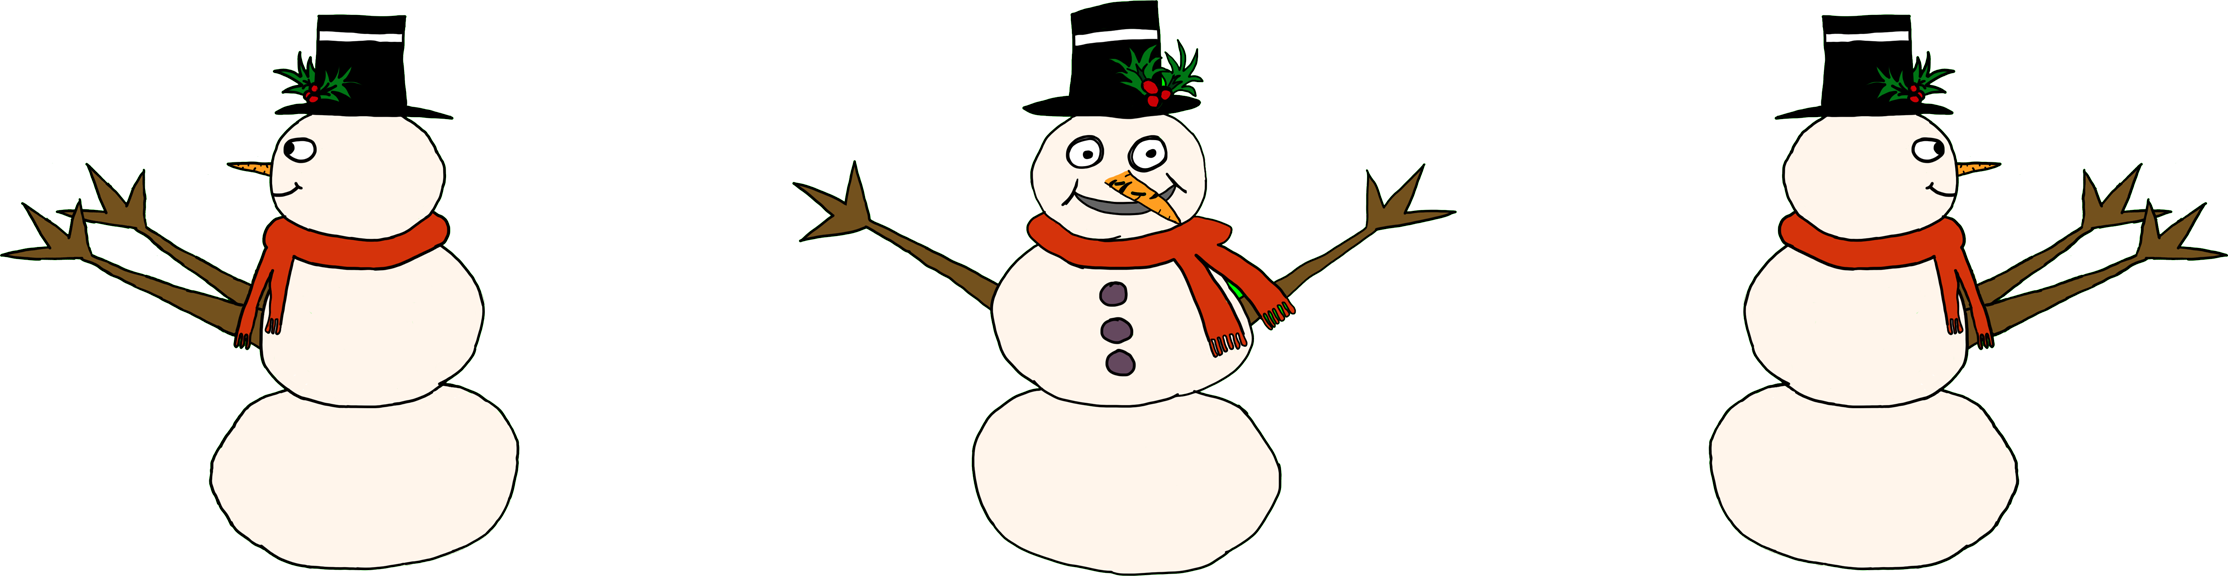
\includegraphics[width=1.00\textwidth]{Pictures/Design/SnowManShowOff.png}
\caption{Picture illustrating 3 different animations for one avatar}
\label{fig:Design_SnowmanAnimation}
\end{figure} 
\section{Sprite sheets}
There are many ways of animating an avatar for use on other platforms. One way is to finalize the animation on beforehand and play the actual footage. This is however not a very efficient way of including an animation as it take up space depending on the file format and size. Ultimately having several animations would slow down the program producing a weak\fixme{Find synonym for weak} output. Instead another solution was taken into considerations.\\
It was decided to create complete sprite sheets, to be implemented in Unity for use of animations. A sprite sheet contain all the images needed to create the full cycle and depending on the movement of the user in front of the installation on the library, the different sprite sheets will be activated. Figure \eqref{fig:Design_PixieBoyWalking} illustrates a complete sprite sheet for a user moving horizontally to the right.
\begin{figure}[htbp]
\centering
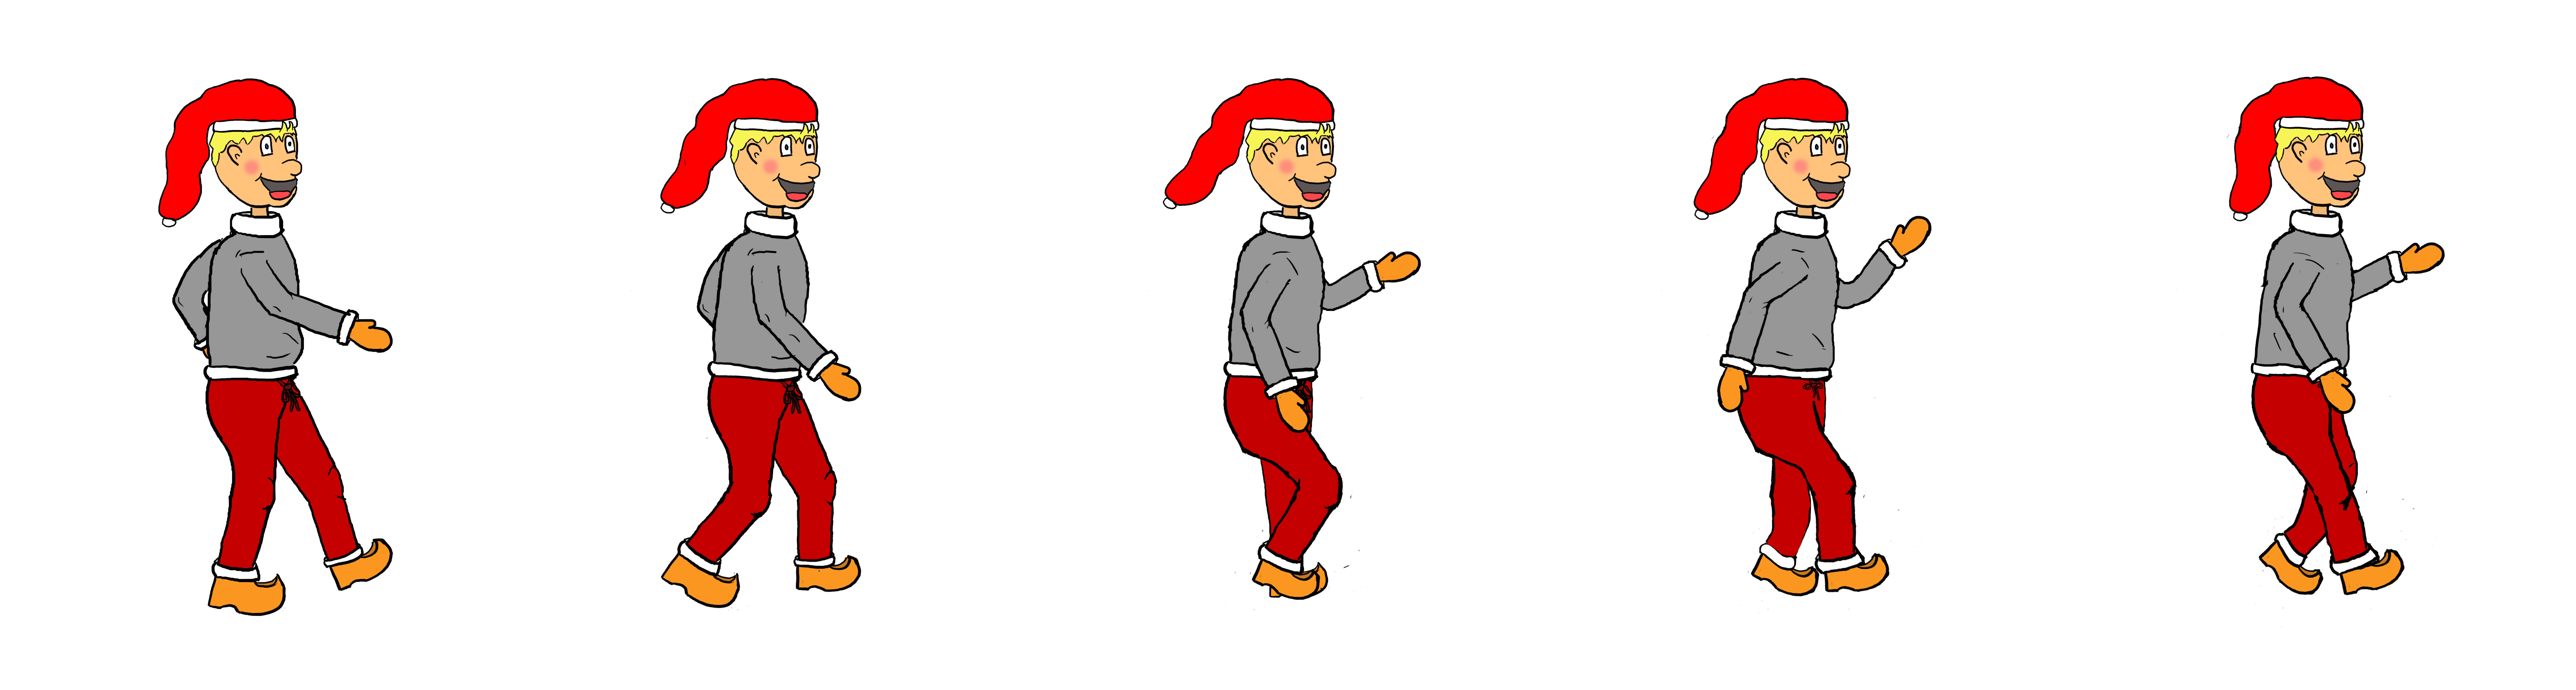
\includegraphics[width=1.00\textwidth]{Pictures/Design/PixieWalking.png}
\caption{Picture illustrating The walk cycle of the pixie boy}
\label{fig:Design_PixieBoyWalking}
\end{figure}





